\documentclass[11pt]{article}
\usepackage[margin=1in]{geometry}
\usepackage{graphicx}
\usepackage{booktabs}
\usepackage{longtable}
\usepackage{array}
\usepackage{pdflscape}
\usepackage{caption}
\usepackage{hyperref}
\usepackage{siunitx}
\usepackage{float}
\hypersetup{colorlinks=true, linkcolor=blue, urlcolor=blue, citecolor=blue}
\sisetup{group-separator={,}, group-minimum-digits=4}

\title{Clausius Beta-Branch Recompute Report}
\author{Generated from \texttt{notebooks/guided\_clausius\_beta\_branch\_recompute.ipynb}}
\date{Generated from saved QMM outputs}

\begin{document}
\maketitle

\begin{abstract}
This package summarizes the saved outputs of the guided Clausius
beta-branch recompute notebook. It collects the asymmetric hadronic
couplings $(a_n, a_{pn}, b_n, b_{pn})$ for every scanned
incompressibility $K_0$, the fixed-$y$ critical-point results
$(T_c, n_c, P_c)$, the beta-equilibrium sound-speed peaks, and the
corresponding raw EOS/profile tables in one clean Overleaf-ready folder.
The copied machine-readable data are stored in \texttt{data/raw/} and
\texttt{data/derived/}.
\end{abstract}

\section{Source and Scope}
The report was built from the saved outputs of:
\begin{itemize}
\item \texttt{notebooks/guided\_clausius\_beta\_branch\_recompute.ipynb}
\item \texttt{results/generated/guided\_clausius\_beta\_branch\_recompute}
\end{itemize}

The scan covers:
\begin{itemize}
\item Clausius mean field with the notebook's asymmetric-beta branch setup
\item both asymmetric branches: \texttt{target\_l} and \texttt{equal\_b}
\item $K_0 = 250, 255, \ldots, 315~\mathrm{MeV}$
\item saved beta-equilibrium profiles, fixed-$y$ profiles, hadronic EOS tables,
      and neutron-star sequences
\end{itemize}

\section{Asymmetric Couplings}
Figure~\ref{fig:fit-c-vs-k0} shows the Clausius parameter $c$, and
Figure~\ref{fig:fit-params} shows the fitted asymmetric couplings across
the full $K_0$ scan. Table~\ref{tab:fit-selected} lists selected points
that are often used as representative cases, while the full machine table
is included in Appendix~\ref{sec:appendix-fit}.

\begin{figure}[H]
  \centering
  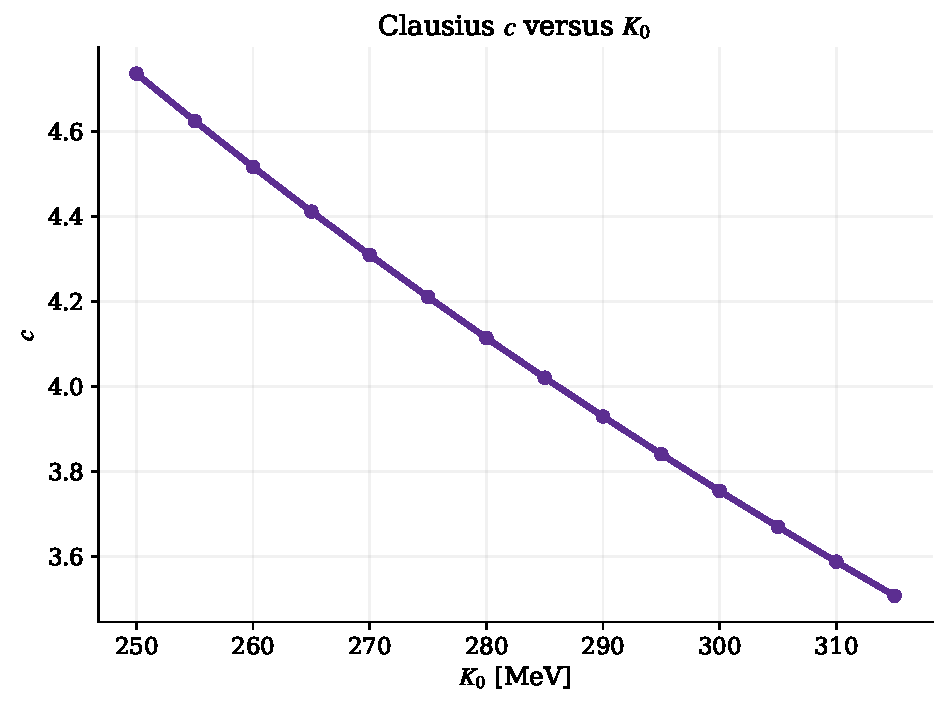
\includegraphics[width=0.62\textwidth]{figures/fit_c_vs_k0.pdf}
  \caption{Clausius parameter $c$ as a function of the requested incompressibility $K_0$. This parameter comes from the common symmetric-matter fit, so the two branches coincide in this plot.}
  \label{fig:fit-c-vs-k0}
\end{figure}

\begin{figure}[H]
  \centering
  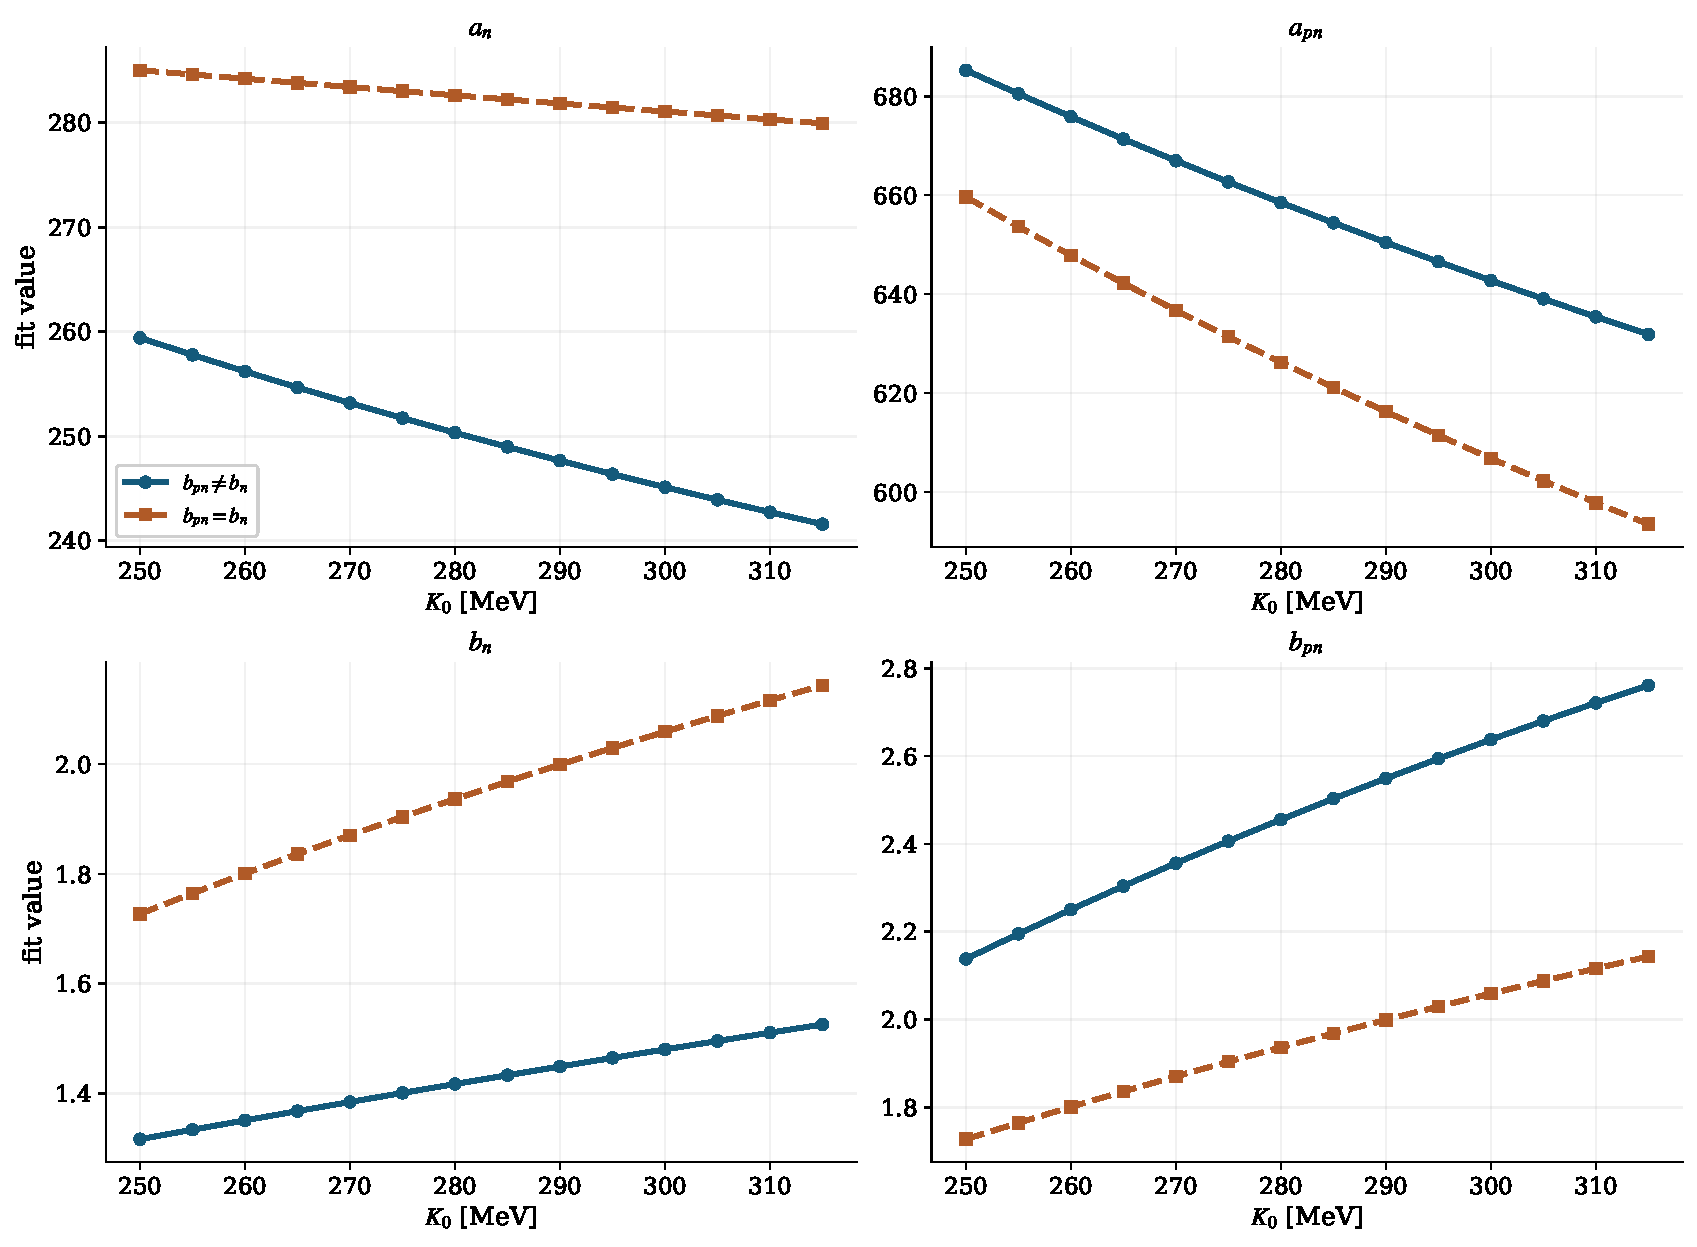
\includegraphics[width=0.96\textwidth]{figures/fit_parameters_vs_k0.pdf}
  \caption{Asymmetric Clausius couplings as functions of the requested incompressibility $K_0$.}
  \label{fig:fit-params}
\end{figure}

\begin{table}[htbp]
        \centering
        \caption{Selected asymmetric-fit couplings from the guided Clausius beta-branch recompute notebook.}
        \label{tab:fit-selected}
        \begin{tabular}{r l r r r r r r}
        \toprule
        $K_0$ & branch & $c$ & $a_n$ & $a_{pn}$ & $b_n$ & $b_{pn}$ & $L$ \\
        \midrule
        250 & $b_{pn} \neq b_n$ & 4.735853 & 259.413733 & 685.241284 & 1.316923 & 2.137819 & 58.900000 \\
250 & $b_{pn} = b_n$ & 4.735853 & 285.021459 & 659.633558 & 1.727371 & 1.727371 & 70.058236 \\
280 & $b_{pn} \neq b_n$ & 4.114108 & 250.336526 & 658.488869 & 1.417423 & 2.455476 & 58.900000 \\
280 & $b_{pn} = b_n$ & 4.114108 & 282.624717 & 626.200678 & 1.936450 & 1.936450 & 74.195002 \\
315 & $b_{pn} \neq b_n$ & 3.507371 & 241.580371 & 631.849247 & 1.525881 & 2.761368 & 58.900000 \\
315 & $b_{pn} = b_n$ & 3.507371 & 279.942373 & 593.487245 & 2.143624 & 2.143624 & 78.732268 \\
        \bottomrule
        \end{tabular}
        \end{table}


\begin{figure}[H]
  \centering
  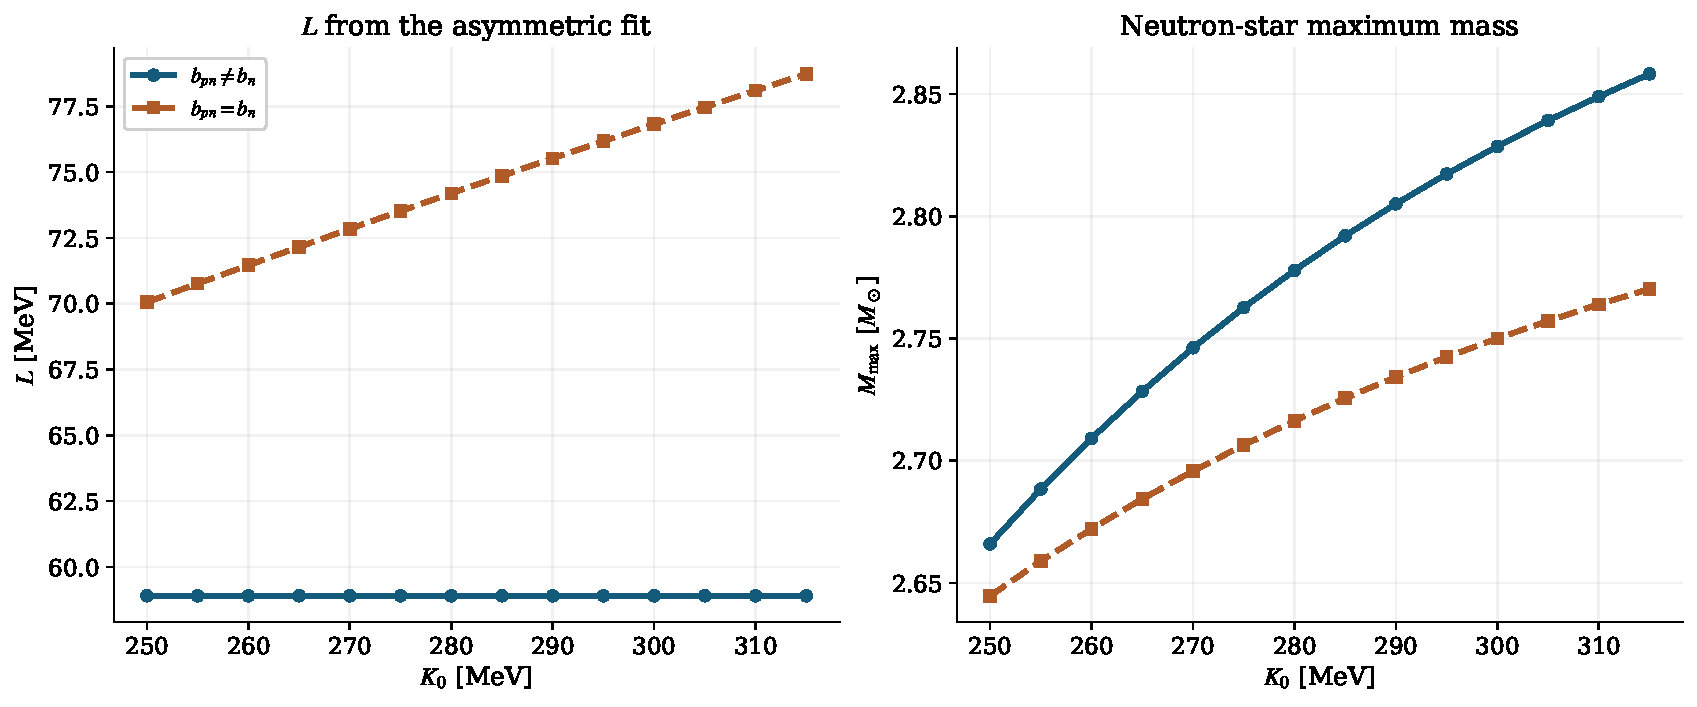
\includegraphics[width=0.96\textwidth]{figures/fit_slope_and_maxmass_vs_k0.pdf}
  \caption{Auxiliary scan diagnostics: fitted symmetry slope $L$ and neutron-star maximum mass.}
  \label{fig:slope-maxmass}
\end{figure}

\section{Fixed-$y$ Critical Points}
Figures~\ref{fig:fixed-y-vs-y} and~\ref{fig:fixed-y-vs-k0} summarize
the fixed-$y$ critical-point families computed from the saved notebook
outputs. The full table of $(K_0, y, T_c, n_c, P_c)$ values is included in
Appendix~\ref{sec:appendix-fixed-y} and in the derived CSV files.

\begin{figure}[H]
  \centering
  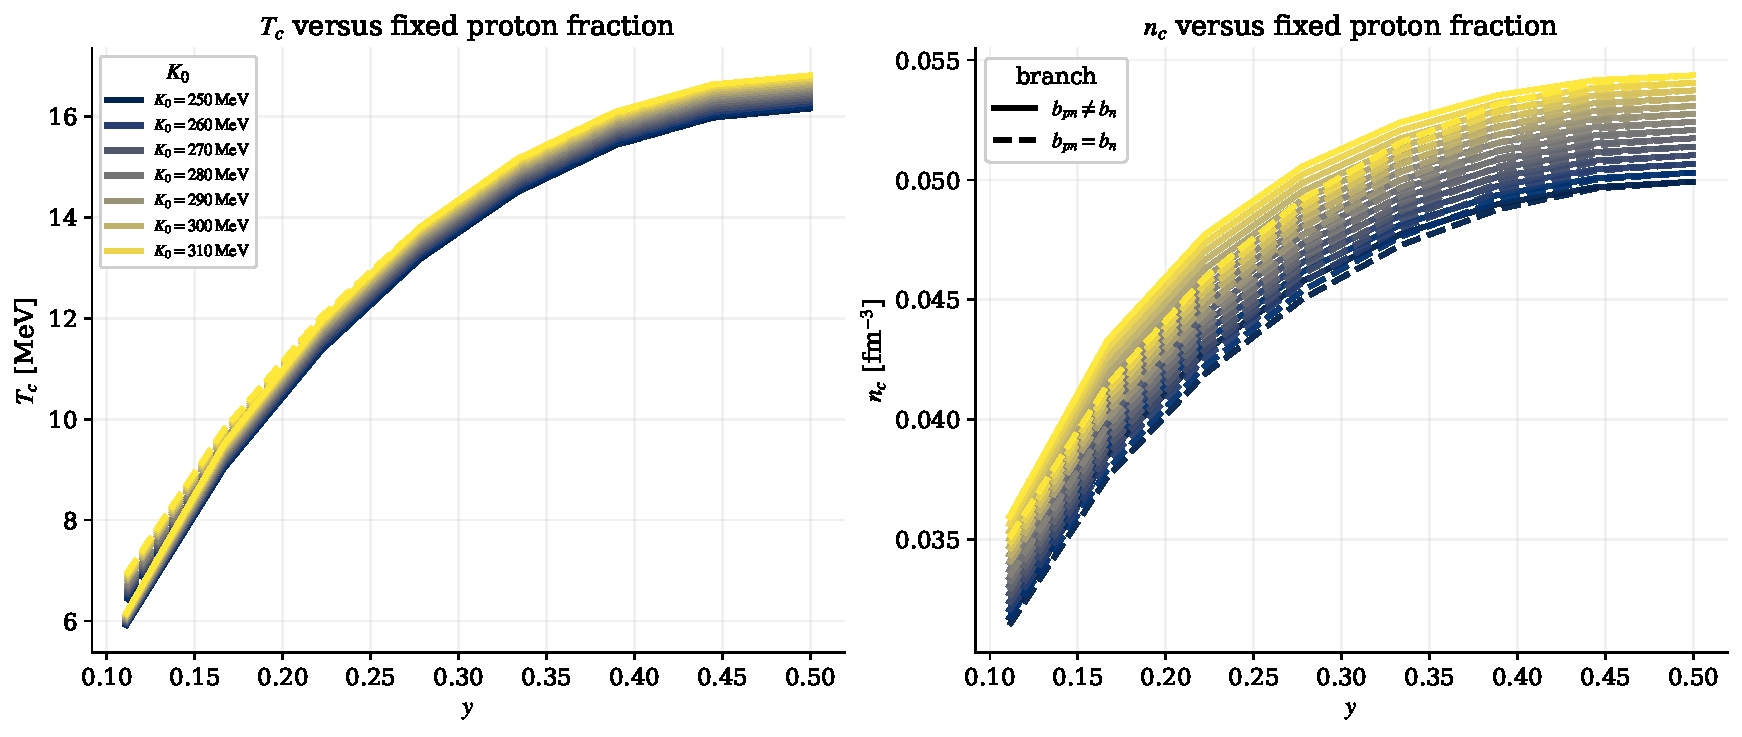
\includegraphics[width=0.95\textwidth]{figures/fixed_y_critical_vs_y.pdf}
  \caption{Critical temperature and critical density versus fixed proton fraction $y$.}
  \label{fig:fixed-y-vs-y}
\end{figure}

\begin{figure}[H]
  \centering
  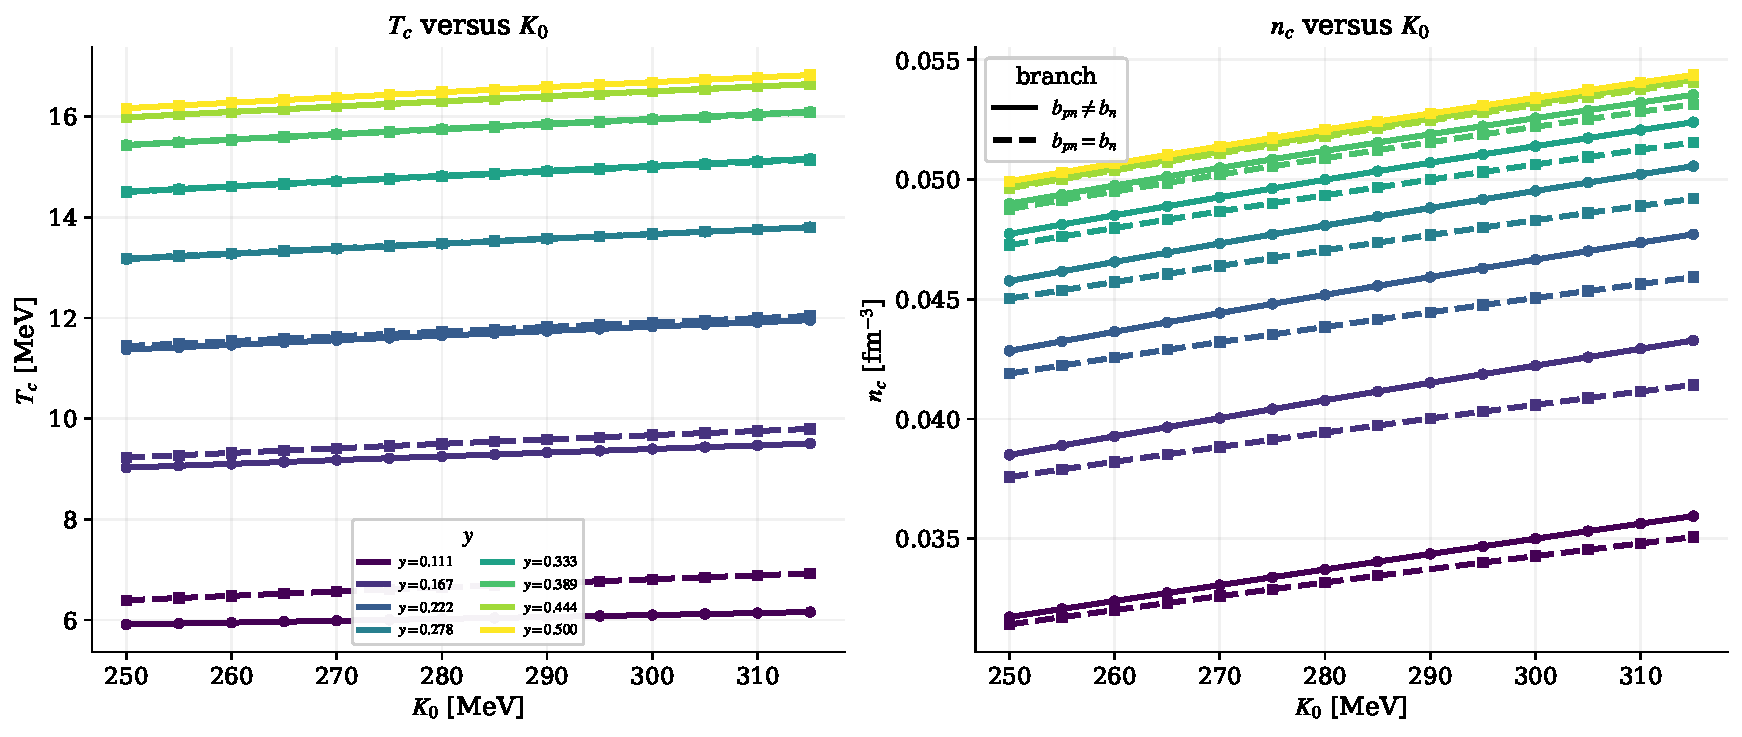
\includegraphics[width=0.95\textwidth]{figures/fixed_y_critical_vs_k0.pdf}
  \caption{Critical temperature and critical density versus incompressibility $K_0$. The right panel gives the requested $K_0$ versus $n_c$ view explicitly.}
  \label{fig:fixed-y-vs-k0}
\end{figure}

\section{Beta-Equilibrium Profiles and EOS}
Figure~\ref{fig:beta-selected} shows representative beta-equilibrium
curves for the selected $K_0 = 250, 280, 315~\mathrm{MeV}$ cases, including
the charge fraction, quark fraction, postprocessed sound speed, the
requested $\varepsilon / \rho_B - m_N$ profile, and the EOS.
The sound-speed peak summary from the notebook-side reconstruction is shown
in Figure~\ref{fig:beta-peak} and tabulated in Appendix~\ref{sec:appendix-beta-peak}.

\begin{figure}[H]
  \centering
  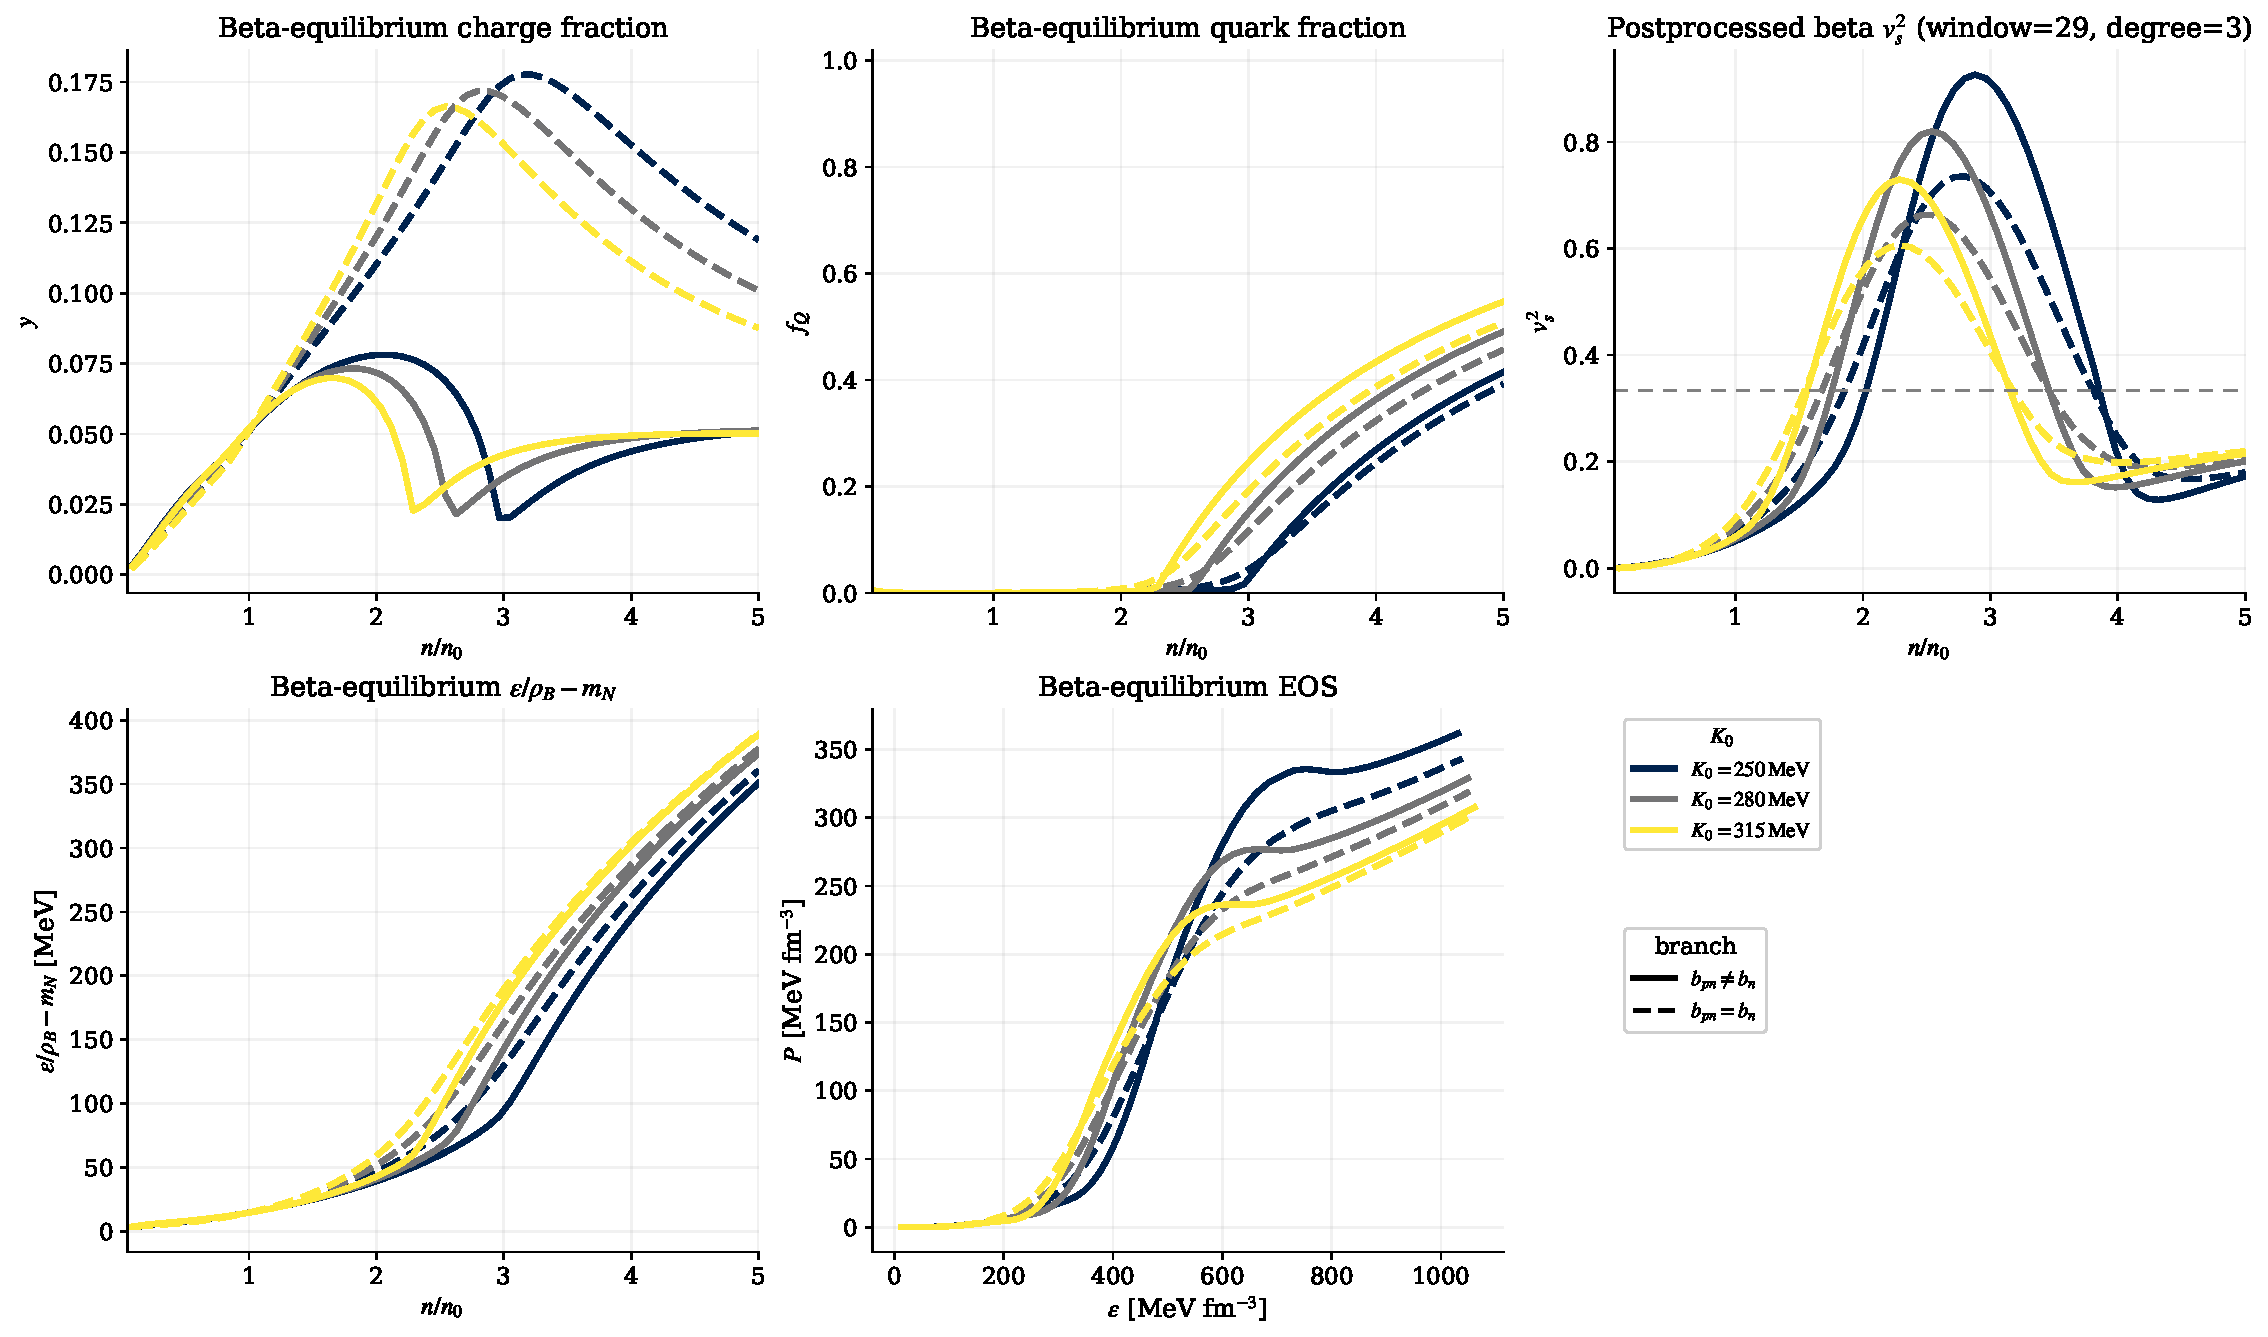
\includegraphics[width=0.97\textwidth]{figures/beta_profiles_selected_k0.pdf}
  \caption{Representative beta-equilibrium profiles, $\varepsilon / \rho_B - m_N$, and EOS from the saved notebook outputs. The sound-speed reconstruction uses the notebook postprocessing choices window=29, degree=3.}
  \label{fig:beta-selected}
\end{figure}

\begin{figure}[H]
  \centering
  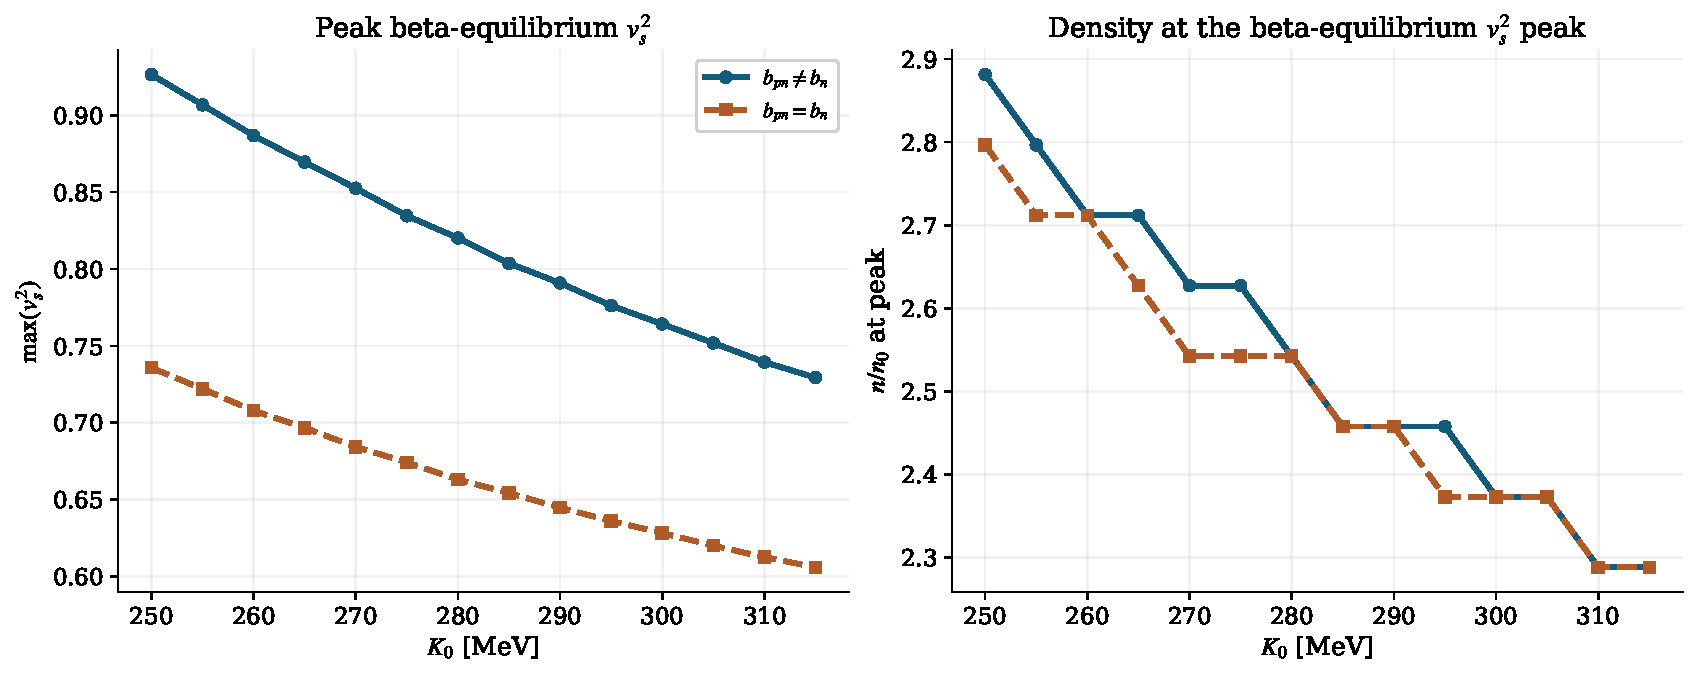
\includegraphics[width=0.95\textwidth]{figures/beta_peak_summary_vs_k0.pdf}
  \caption{Summary of the beta-equilibrium sound-speed peaks from the notebook postprocessing step.}
  \label{fig:beta-peak}
\end{figure}

\section{Data Layout}
The project contains both copied raw outputs and derived summary files:
\begin{itemize}
\item \texttt{data/raw/}: per-run CSV and JSON files copied from the source notebook output tree
\item \texttt{data/derived/fit\_parameters\_all.csv}: combined asymmetric-fit table
\item \texttt{data/derived/fixed\_y\_critical\_points\_all.csv}: combined fixed-$y$ critical-point table
\item \texttt{data/derived/beta\_sound\_speed\_peak\_summary.csv}: peak $v_s^2$ summary
\item \texttt{data/derived/neutron\_star\_maxima.csv}: neutron-star maximum-mass summary
\end{itemize}

\appendix

\section{Full Asymmetric-Fit Table}
\label{sec:appendix-fit}
\begin{longtable}{r l r r r r r r r}
        \caption{Full asymmetric-fit parameter table copied from the notebook scan.}\label{tab:fit-all} \\
        \toprule
        $K_0$ & branch & $c$ & $a_n$ & $a_{pn}$ & $b_n$ & $b_{pn}$ & $J$ & $L$ \\
        \midrule
        \endfirsthead
        \caption[]{Full asymmetric-fit parameter table copied from the notebook scan. (continued)} \\
        \toprule
        $K_0$ & branch & $c$ & $a_n$ & $a_{pn}$ & $b_n$ & $b_{pn}$ & $J$ & $L$ \\
        \midrule
        \endhead
        \midrule
        \multicolumn{9}{r}{Continued on next page} \\
        \midrule
        \endfoot
        \bottomrule
        \endlastfoot
        250 & $b_{pn} \neq b_n$ & 4.735852852 & 259.413733 & 685.241284 & 1.316923 & 2.137819 & 32.500000 & 58.900000 \\
250 & $b_{pn} = b_n$ & 4.735852852 & 285.021459 & 659.633558 & 1.727371 & 1.727371 & 32.500000 & 70.058236 \\
255 & $b_{pn} \neq b_n$ & 4.624418225 & 257.779723 & 680.484732 & 1.334208 & 2.195018 & 32.500000 & 58.900000 \\
255 & $b_{pn} = b_n$ & 4.624418225 & 284.616705 & 653.647750 & 1.764613 & 1.764613 & 32.500000 & 70.765359 \\
260 & $b_{pn} \neq b_n$ & 4.516312367 & 256.197400 & 675.854641 & 1.351272 & 2.250404 & 32.500000 & 58.900000 \\
260 & $b_{pn} = b_n$ & 4.516312367 & 284.213883 & 647.838157 & 1.800838 & 1.800838 & 32.500000 & 71.465148 \\
265 & $b_{pn} \neq b_n$ & 4.411374181 & 254.664218 & 671.345246 & 1.368119 & 2.304064 & 32.500000 & 58.900000 \\
265 & $b_{pn} = b_n$ & 4.411374181 & 283.813148 & 642.196316 & 1.836091 & 1.836091 & 32.500000 & 72.157813 \\
270 & $b_{pn} \neq b_n$ & 4.309453024 & 253.177801 & 666.951141 & 1.384757 & 2.356079 & 32.500000 & 58.900000 \\
270 & $b_{pn} = b_n$ & 4.309453024 & 283.414635 & 636.714307 & 1.870418 & 1.870418 & 32.500000 & 72.843552 \\
275 & $b_{pn} \neq b_n$ & 4.210408302 & 251.735930 & 662.667268 & 1.401189 & 2.406526 & 32.500000 & 58.900000 \\
275 & $b_{pn} = b_n$ & 4.210408302 & 283.018458 & 631.384740 & 1.903858 & 1.903858 & 32.500000 & 73.522554 \\
280 & $b_{pn} \neq b_n$ & 4.114108114 & 250.336526 & 658.488869 & 1.417423 & 2.455476 & 32.500000 & 58.900000 \\
280 & $b_{pn} = b_n$ & 4.114108114 & 282.624717 & 626.200678 & 1.936450 & 1.936450 & 32.500000 & 74.195002 \\
285 & $b_{pn} \neq b_n$ & 4.020429107 & 248.977643 & 654.411483 & 1.433463 & 2.502996 & 32.500000 & 58.900000 \\
285 & $b_{pn} = b_n$ & 4.020429107 & 282.233497 & 621.155629 & 1.968230 & 1.968230 & 32.500000 & 74.861069 \\
290 & $b_{pn} \neq b_n$ & 3.929255287 & 247.657455 & 650.430903 & 1.449313 & 2.549149 & 32.500000 & 58.900000 \\
290 & $b_{pn} = b_n$ & 3.929255287 & 281.844868 & 616.243490 & 1.999231 & 1.999231 & 32.500000 & 75.520919 \\
295 & $b_{pn} \neq b_n$ & 3.840477834 & 246.374246 & 646.543177 & 1.464979 & 2.593995 & 32.500000 & 58.900000 \\
295 & $b_{pn} = b_n$ & 3.840477834 & 281.458892 & 611.458531 & 2.029487 & 2.029487 & 32.500000 & 76.174713 \\
300 & $b_{pn} \neq b_n$ & 3.753994379 & 245.126408 & 642.744572 & 1.480464 & 2.637588 & 32.500000 & 58.900000 \\
300 & $b_{pn} = b_n$ & 3.753994379 & 281.075617 & 606.795362 & 2.059026 & 2.059026 & 32.500000 & 76.822602 \\
305 & $b_{pn} \neq b_n$ & 3.669708496 & 243.912420 & 639.031568 & 1.495773 & 2.679982 & 32.500000 & 58.900000 \\
305 & $b_{pn} = b_n$ & 3.669708496 & 280.695085 & 602.248903 & 2.087878 & 2.087878 & 32.500000 & 77.464731 \\
310 & $b_{pn} \neq b_n$ & 3.587529400 & 242.730857 & 635.400841 & 1.510911 & 2.721226 & 32.500000 & 58.900000 \\
310 & $b_{pn} = b_n$ & 3.587529400 & 280.317329 & 597.814370 & 2.116069 & 2.116069 & 32.500000 & 78.101242 \\
315 & $b_{pn} \neq b_n$ & 3.507371383 & 241.580371 & 631.849247 & 1.525881 & 2.761368 & 32.500000 & 58.900000 \\
315 & $b_{pn} = b_n$ & 3.507371383 & 279.942373 & 593.487245 & 2.143624 & 2.143624 & 32.500000 & 78.732268 \\
        \end{longtable}


\section{Full Fixed-$y$ Critical-Point Table}
\label{sec:appendix-fixed-y}
\begin{longtable}{l r r r r r}
        \caption{Full fixed-$y$ critical-point table derived from the saved notebook outputs.}\label{tab:fixed-y-all} \\
        \toprule
        branch & $K_0$ & $y$ & $T_c$ & $n_c$ & $P_c$ \\
        \midrule
        \endfirsthead
        \caption[]{Full fixed-$y$ critical-point table derived from the saved notebook outputs. (continued)} \\
        \toprule
        branch & $K_0$ & $y$ & $T_c$ & $n_c$ & $P_c$ \\
        \midrule
        \endhead
        \midrule
        \multicolumn{6}{r}{Continued on next page} \\
        \midrule
        \endfoot
        \bottomrule
        \endlastfoot
        $b_{pn} \neq b_n$ & 250 & 0.111111 & 5.913821 & 0.031727 & 0.058358 \\
$b_{pn} \neq b_n$ & 250 & 0.166667 & 9.026804 & 0.038500 & 0.106647 \\
$b_{pn} \neq b_n$ & 250 & 0.222222 & 11.369632 & 0.042843 & 0.148202 \\
$b_{pn} \neq b_n$ & 250 & 0.277778 & 13.166415 & 0.045765 & 0.182247 \\
$b_{pn} \neq b_n$ & 250 & 0.333333 & 14.505498 & 0.047730 & 0.208550 \\
$b_{pn} \neq b_n$ & 250 & 0.388889 & 15.434808 & 0.048992 & 0.227176 \\
$b_{pn} \neq b_n$ & 250 & 0.444444 & 15.982386 & 0.049698 & 0.238270 \\
$b_{pn} \neq b_n$ & 250 & 0.500000 & 16.163319 & 0.049925 & 0.241953 \\
$b_{pn} \neq b_n$ & 255 & 0.111111 & 5.931709 & 0.032064 & 0.059249 \\
$b_{pn} \neq b_n$ & 255 & 0.166667 & 9.064686 & 0.038890 & 0.108392 \\
$b_{pn} \neq b_n$ & 255 & 0.222222 & 11.417146 & 0.043245 & 0.150566 \\
$b_{pn} \neq b_n$ & 255 & 0.277778 & 13.218606 & 0.046165 & 0.185041 \\
$b_{pn} \neq b_n$ & 255 & 0.333333 & 14.559708 & 0.048121 & 0.211631 \\
$b_{pn} \neq b_n$ & 255 & 0.388889 & 15.489692 & 0.049374 & 0.230434 \\
$b_{pn} \neq b_n$ & 255 & 0.444444 & 16.037394 & 0.050074 & 0.241623 \\
$b_{pn} \neq b_n$ & 255 & 0.500000 & 16.218324 & 0.050299 & 0.245337 \\
$b_{pn} \neq b_n$ & 260 & 0.111111 & 5.949795 & 0.032399 & 0.060144 \\
$b_{pn} \neq b_n$ & 260 & 0.166667 & 9.102380 & 0.039276 & 0.110137 \\
$b_{pn} \neq b_n$ & 260 & 0.222222 & 11.464215 & 0.043643 & 0.152926 \\
$b_{pn} \neq b_n$ & 260 & 0.277778 & 13.270179 & 0.046559 & 0.187826 \\
$b_{pn} \neq b_n$ & 260 & 0.333333 & 14.613198 & 0.048506 & 0.214697 \\
$b_{pn} \neq b_n$ & 260 & 0.388889 & 15.543801 & 0.049750 & 0.233674 \\
$b_{pn} \neq b_n$ & 260 & 0.444444 & 16.091599 & 0.050444 & 0.244957 \\
$b_{pn} \neq b_n$ & 260 & 0.500000 & 16.272518 & 0.050667 & 0.248700 \\
$b_{pn} \neq b_n$ & 265 & 0.111111 & 5.968073 & 0.032732 & 0.061043 \\
$b_{pn} \neq b_n$ & 265 & 0.166667 & 9.139898 & 0.039658 & 0.111882 \\
$b_{pn} \neq b_n$ & 265 & 0.222222 & 11.510849 & 0.044035 & 0.155281 \\
$b_{pn} \neq b_n$ & 265 & 0.277778 & 13.321158 & 0.046947 & 0.190601 \\
$b_{pn} \neq b_n$ & 265 & 0.333333 & 14.665993 & 0.048885 & 0.217749 \\
$b_{pn} \neq b_n$ & 265 & 0.388889 & 15.597159 & 0.050120 & 0.236896 \\
$b_{pn} \neq b_n$ & 265 & 0.444444 & 16.145029 & 0.050808 & 0.248272 \\
$b_{pn} \neq b_n$ & 265 & 0.500000 & 16.325928 & 0.051029 & 0.252043 \\
$b_{pn} \neq b_n$ & 270 & 0.111111 & 5.986536 & 0.033062 & 0.061946 \\
$b_{pn} \neq b_n$ & 270 & 0.166667 & 9.177220 & 0.040036 & 0.113629 \\
$b_{pn} \neq b_n$ & 270 & 0.222222 & 11.557061 & 0.044423 & 0.157631 \\
$b_{pn} \neq b_n$ & 270 & 0.277778 & 13.371563 & 0.047330 & 0.193367 \\
$b_{pn} \neq b_n$ & 270 & 0.333333 & 14.718115 & 0.049259 & 0.220787 \\
$b_{pn} \neq b_n$ & 270 & 0.388889 & 15.649792 & 0.050485 & 0.240102 \\
$b_{pn} \neq b_n$ & 270 & 0.444444 & 16.197708 & 0.051166 & 0.251567 \\
$b_{pn} \neq b_n$ & 270 & 0.500000 & 16.378581 & 0.051385 & 0.255367 \\
$b_{pn} \neq b_n$ & 275 & 0.111111 & 6.005180 & 0.033390 & 0.062852 \\
$b_{pn} \neq b_n$ & 275 & 0.166667 & 9.214371 & 0.040410 & 0.115376 \\
$b_{pn} \neq b_n$ & 275 & 0.222222 & 11.602857 & 0.044806 & 0.159978 \\
$b_{pn} \neq b_n$ & 275 & 0.277778 & 13.421399 & 0.047708 & 0.196123 \\
$b_{pn} \neq b_n$ & 275 & 0.333333 & 14.769580 & 0.049627 & 0.223811 \\
$b_{pn} \neq b_n$ & 275 & 0.388889 & 15.701722 & 0.050844 & 0.243291 \\
$b_{pn} \neq b_n$ & 275 & 0.444444 & 16.249660 & 0.051520 & 0.254845 \\
$b_{pn} \neq b_n$ & 275 & 0.500000 & 16.430501 & 0.051736 & 0.258672 \\
$b_{pn} \neq b_n$ & 280 & 0.111111 & 6.023998 & 0.033716 & 0.063762 \\
$b_{pn} \neq b_n$ & 280 & 0.166667 & 9.251347 & 0.040781 & 0.117124 \\
$b_{pn} \neq b_n$ & 280 & 0.222222 & 11.648251 & 0.045185 & 0.162320 \\
$b_{pn} \neq b_n$ & 280 & 0.277778 & 13.470686 & 0.048081 & 0.198870 \\
$b_{pn} \neq b_n$ & 280 & 0.333333 & 14.820412 & 0.049990 & 0.226822 \\
$b_{pn} \neq b_n$ & 280 & 0.388889 & 15.752967 & 0.051198 & 0.246464 \\
$b_{pn} \neq b_n$ & 280 & 0.444444 & 16.300916 & 0.051867 & 0.258105 \\
$b_{pn} \neq b_n$ & 280 & 0.500000 & 16.481711 & 0.052081 & 0.261959 \\
$b_{pn} \neq b_n$ & 285 & 0.111111 & 6.042987 & 0.034040 & 0.064676 \\
$b_{pn} \neq b_n$ & 285 & 0.166667 & 9.288150 & 0.041148 & 0.118873 \\
$b_{pn} \neq b_n$ & 285 & 0.222222 & 11.693251 & 0.045559 & 0.164658 \\
$b_{pn} \neq b_n$ & 285 & 0.277778 & 13.519442 & 0.048449 & 0.201608 \\
$b_{pn} \neq b_n$ & 285 & 0.333333 & 14.870627 & 0.050348 & 0.229819 \\
$b_{pn} \neq b_n$ & 285 & 0.388889 & 15.803554 & 0.051547 & 0.249621 \\
$b_{pn} \neq b_n$ & 285 & 0.444444 & 16.351480 & 0.052210 & 0.261347 \\
$b_{pn} \neq b_n$ & 285 & 0.500000 & 16.532233 & 0.052422 & 0.265228 \\
$b_{pn} \neq b_n$ & 290 & 0.111111 & 6.062139 & 0.034362 & 0.065594 \\
$b_{pn} \neq b_n$ & 290 & 0.166667 & 9.324781 & 0.041511 & 0.120623 \\
$b_{pn} \neq b_n$ & 290 & 0.222222 & 11.737866 & 0.045928 & 0.166992 \\
$b_{pn} \neq b_n$ & 290 & 0.277778 & 13.567676 & 0.048812 & 0.204337 \\
$b_{pn} \neq b_n$ & 290 & 0.333333 & 14.920243 & 0.050701 & 0.232804 \\
$b_{pn} \neq b_n$ & 290 & 0.388889 & 15.853499 & 0.051891 & 0.252762 \\
$b_{pn} \neq b_n$ & 290 & 0.444444 & 16.401387 & 0.052547 & 0.264572 \\
$b_{pn} \neq b_n$ & 290 & 0.500000 & 16.582089 & 0.052757 & 0.268479 \\
$b_{pn} \neq b_n$ & 295 & 0.111111 & 6.081450 & 0.034682 & 0.066516 \\
$b_{pn} \neq b_n$ & 295 & 0.166667 & 9.361243 & 0.041871 & 0.122373 \\
$b_{pn} \neq b_n$ & 295 & 0.222222 & 11.782105 & 0.046294 & 0.169322 \\
$b_{pn} \neq b_n$ & 295 & 0.277778 & 13.615404 & 0.049170 & 0.207057 \\
$b_{pn} \neq b_n$ & 295 & 0.333333 & 14.969284 & 0.051049 & 0.235777 \\
$b_{pn} \neq b_n$ & 295 & 0.388889 & 15.902821 & 0.052229 & 0.255888 \\
$b_{pn} \neq b_n$ & 295 & 0.444444 & 16.450652 & 0.052880 & 0.267780 \\
$b_{pn} \neq b_n$ & 295 & 0.500000 & 16.631298 & 0.053088 & 0.271713 \\
$b_{pn} \neq b_n$ & 300 & 0.111111 & 6.100916 & 0.035000 & 0.067442 \\
$b_{pn} \neq b_n$ & 300 & 0.166667 & 9.397539 & 0.042228 & 0.124125 \\
$b_{pn} \neq b_n$ & 300 & 0.222222 & 11.825974 & 0.046655 & 0.171648 \\
$b_{pn} \neq b_n$ & 300 & 0.277778 & 13.662640 & 0.049524 & 0.209769 \\
$b_{pn} \neq b_n$ & 300 & 0.333333 & 15.017752 & 0.051392 & 0.238738 \\
$b_{pn} \neq b_n$ & 300 & 0.388889 & 15.951539 & 0.052563 & 0.258999 \\
$b_{pn} \neq b_n$ & 300 & 0.444444 & 16.499291 & 0.053208 & 0.270971 \\
$b_{pn} \neq b_n$ & 300 & 0.500000 & 16.679880 & 0.053413 & 0.274930 \\
$b_{pn} \neq b_n$ & 305 & 0.111111 & 6.120532 & 0.035316 & 0.068373 \\
$b_{pn} \neq b_n$ & 305 & 0.166667 & 9.433673 & 0.042581 & 0.125878 \\
$b_{pn} \neq b_n$ & 305 & 0.222222 & 11.869476 & 0.047012 & 0.173970 \\
$b_{pn} \neq b_n$ & 305 & 0.277778 & 13.709392 & 0.049873 & 0.212473 \\
$b_{pn} \neq b_n$ & 305 & 0.333333 & 15.065668 & 0.051731 & 0.241686 \\
$b_{pn} \neq b_n$ & 305 & 0.388889 & 15.999668 & 0.052893 & 0.262096 \\
$b_{pn} \neq b_n$ & 305 & 0.444444 & 16.547329 & 0.053531 & 0.274147 \\
$b_{pn} \neq b_n$ & 305 & 0.500000 & 16.727853 & 0.053735 & 0.278130 \\
$b_{pn} \neq b_n$ & 310 & 0.111111 & 6.140293 & 0.035630 & 0.069307 \\
$b_{pn} \neq b_n$ & 310 & 0.166667 & 9.469642 & 0.042931 & 0.127632 \\
$b_{pn} \neq b_n$ & 310 & 0.222222 & 11.912643 & 0.047365 & 0.176289 \\
$b_{pn} \neq b_n$ & 310 & 0.277778 & 13.755677 & 0.050218 & 0.215168 \\
$b_{pn} \neq b_n$ & 310 & 0.333333 & 15.113047 & 0.052065 & 0.244622 \\
$b_{pn} \neq b_n$ & 310 & 0.388889 & 16.047233 & 0.053218 & 0.265179 \\
$b_{pn} \neq b_n$ & 310 & 0.444444 & 16.594785 & 0.053850 & 0.277308 \\
$b_{pn} \neq b_n$ & 310 & 0.500000 & 16.775235 & 0.054051 & 0.281315 \\
$b_{pn} \neq b_n$ & 315 & 0.111111 & 6.160196 & 0.035943 & 0.070245 \\
$b_{pn} \neq b_n$ & 315 & 0.166667 & 9.505452 & 0.043278 & 0.129387 \\
$b_{pn} \neq b_n$ & 315 & 0.222222 & 11.955455 & 0.047714 & 0.178604 \\
$b_{pn} \neq b_n$ & 315 & 0.277778 & 13.801501 & 0.050559 & 0.217855 \\
$b_{pn} \neq b_n$ & 315 & 0.333333 & 15.159904 & 0.052395 & 0.247547 \\
$b_{pn} \neq b_n$ & 315 & 0.388889 & 16.094239 & 0.053538 & 0.268247 \\
$b_{pn} \neq b_n$ & 315 & 0.444444 & 16.641668 & 0.054164 & 0.280452 \\
$b_{pn} \neq b_n$ & 315 & 0.500000 & 16.822042 & 0.054364 & 0.284483 \\
$b_{pn} = b_n$ & 250 & 0.111111 & 6.394464 & 0.031419 & 0.062741 \\
$b_{pn} = b_n$ & 250 & 0.166667 & 9.226035 & 0.037576 & 0.106930 \\
$b_{pn} = b_n$ & 250 & 0.222222 & 11.439733 & 0.041896 & 0.146473 \\
$b_{pn} = b_n$ & 250 & 0.277778 & 13.179416 & 0.045025 & 0.180065 \\
$b_{pn} = b_n$ & 250 & 0.333333 & 14.499756 & 0.047261 & 0.206837 \\
$b_{pn} = b_n$ & 250 & 0.388889 & 15.428283 & 0.048768 & 0.226258 \\
$b_{pn} = b_n$ & 250 & 0.444444 & 15.980173 & 0.049640 & 0.238017 \\
$b_{pn} = b_n$ & 250 & 0.500000 & 16.163319 & 0.049925 & 0.241953 \\
$b_{pn} = b_n$ & 255 & 0.111111 & 6.438532 & 0.031721 & 0.063896 \\
$b_{pn} = b_n$ & 255 & 0.166667 & 9.273288 & 0.037896 & 0.108635 \\
$b_{pn} = b_n$ & 255 & 0.222222 & 11.489533 & 0.042232 & 0.148665 \\
$b_{pn} = b_n$ & 255 & 0.277778 & 13.231163 & 0.045375 & 0.182672 \\
$b_{pn} = b_n$ & 255 & 0.333333 & 14.552953 & 0.047622 & 0.209778 \\
$b_{pn} = b_n$ & 255 & 0.388889 & 15.482491 & 0.049136 & 0.229443 \\
$b_{pn} = b_n$ & 255 & 0.444444 & 16.034981 & 0.050012 & 0.241350 \\
$b_{pn} = b_n$ & 255 & 0.500000 & 16.218324 & 0.050299 & 0.245337 \\
$b_{pn} = b_n$ & 260 & 0.111111 & 6.482032 & 0.032018 & 0.065048 \\
$b_{pn} = b_n$ & 260 & 0.166667 & 9.319904 & 0.038212 & 0.110333 \\
$b_{pn} = b_n$ & 260 & 0.222222 & 11.538638 & 0.042564 & 0.150846 \\
$b_{pn} = b_n$ & 260 & 0.277778 & 13.282170 & 0.045719 & 0.185265 \\
$b_{pn} = b_n$ & 260 & 0.333333 & 14.605384 & 0.047976 & 0.212702 \\
$b_{pn} = b_n$ & 260 & 0.388889 & 15.535907 & 0.049498 & 0.232609 \\
$b_{pn} = b_n$ & 260 & 0.444444 & 16.088981 & 0.050378 & 0.244664 \\
$b_{pn} = b_n$ & 260 & 0.500000 & 16.272518 & 0.050667 & 0.248700 \\
$b_{pn} = b_n$ & 265 & 0.111111 & 6.524984 & 0.032312 & 0.066198 \\
$b_{pn} = b_n$ & 265 & 0.166667 & 9.365905 & 0.038523 & 0.112025 \\
$b_{pn} = b_n$ & 265 & 0.222222 & 11.587070 & 0.042890 & 0.153017 \\
$b_{pn} = b_n$ & 265 & 0.277778 & 13.332465 & 0.046059 & 0.187845 \\
$b_{pn} = b_n$ & 265 & 0.333333 & 14.657067 & 0.048326 & 0.215610 \\
$b_{pn} = b_n$ & 265 & 0.388889 & 15.588556 & 0.049854 & 0.235757 \\
$b_{pn} = b_n$ & 265 & 0.444444 & 16.142202 & 0.050739 & 0.247958 \\
$b_{pn} = b_n$ & 265 & 0.500000 & 16.325928 & 0.051029 & 0.252043 \\
$b_{pn} = b_n$ & 270 & 0.111111 & 6.567398 & 0.032602 & 0.067346 \\
$b_{pn} = b_n$ & 270 & 0.166667 & 9.411305 & 0.038830 & 0.113711 \\
$b_{pn} = b_n$ & 270 & 0.222222 & 11.634851 & 0.043212 & 0.155178 \\
$b_{pn} = b_n$ & 270 & 0.277778 & 13.382063 & 0.046393 & 0.190411 \\
$b_{pn} = b_n$ & 270 & 0.333333 & 14.708029 & 0.048669 & 0.218502 \\
$b_{pn} = b_n$ & 270 & 0.388889 & 15.640464 & 0.050205 & 0.238888 \\
$b_{pn} = b_n$ & 270 & 0.444444 & 16.194669 & 0.051094 & 0.251234 \\
$b_{pn} = b_n$ & 270 & 0.500000 & 16.378581 & 0.051385 & 0.255367 \\
$b_{pn} = b_n$ & 275 & 0.111111 & 6.609299 & 0.032889 & 0.068493 \\
$b_{pn} = b_n$ & 275 & 0.166667 & 9.456125 & 0.039133 & 0.115390 \\
$b_{pn} = b_n$ & 275 & 0.222222 & 11.682003 & 0.043530 & 0.157329 \\
$b_{pn} = b_n$ & 275 & 0.277778 & 13.430998 & 0.046722 & 0.192964 \\
$b_{pn} = b_n$ & 275 & 0.333333 & 14.758294 & 0.049008 & 0.221379 \\
$b_{pn} = b_n$ & 275 & 0.388889 & 15.691654 & 0.050551 & 0.242000 \\
$b_{pn} = b_n$ & 275 & 0.444444 & 16.246408 & 0.051443 & 0.254491 \\
$b_{pn} = b_n$ & 275 & 0.500000 & 16.430501 & 0.051736 & 0.258672 \\
$b_{pn} = b_n$ & 280 & 0.111111 & 6.650699 & 0.033172 & 0.069637 \\
$b_{pn} = b_n$ & 280 & 0.166667 & 9.500383 & 0.039432 & 0.117063 \\
$b_{pn} = b_n$ & 280 & 0.222222 & 11.728543 & 0.043843 & 0.159471 \\
$b_{pn} = b_n$ & 280 & 0.277778 & 13.479285 & 0.047047 & 0.195505 \\
$b_{pn} = b_n$ & 280 & 0.333333 & 14.807883 & 0.049342 & 0.224240 \\
$b_{pn} = b_n$ & 280 & 0.388889 & 15.742150 & 0.050891 & 0.245096 \\
$b_{pn} = b_n$ & 280 & 0.444444 & 16.297447 & 0.051788 & 0.257730 \\
$b_{pn} = b_n$ & 280 & 0.500000 & 16.481711 & 0.052081 & 0.261959 \\
$b_{pn} = b_n$ & 285 & 0.111111 & 6.691613 & 0.033452 & 0.070779 \\
$b_{pn} = b_n$ & 285 & 0.166667 & 9.544095 & 0.039727 & 0.118731 \\
$b_{pn} = b_n$ & 285 & 0.222222 & 11.774492 & 0.044152 & 0.161603 \\
$b_{pn} = b_n$ & 285 & 0.277778 & 13.526952 & 0.047367 & 0.198033 \\
$b_{pn} = b_n$ & 285 & 0.333333 & 14.856821 & 0.049671 & 0.227086 \\
$b_{pn} = b_n$ & 285 & 0.388889 & 15.791970 & 0.051226 & 0.248175 \\
$b_{pn} = b_n$ & 285 & 0.444444 & 16.347793 & 0.052127 & 0.260951 \\
$b_{pn} = b_n$ & 285 & 0.500000 & 16.532233 & 0.052422 & 0.265228 \\
$b_{pn} = b_n$ & 290 & 0.166667 & 9.587279 & 0.040019 & 0.120393 \\
$b_{pn} = b_n$ & 290 & 0.222222 & 11.819867 & 0.044456 & 0.163726 \\
$b_{pn} = b_n$ & 290 & 0.277778 & 13.574004 & 0.047683 & 0.200549 \\
$b_{pn} = b_n$ & 290 & 0.333333 & 14.905119 & 0.049995 & 0.229918 \\
$b_{pn} = b_n$ & 290 & 0.388889 & 15.841140 & 0.051557 & 0.251238 \\
$b_{pn} = b_n$ & 290 & 0.444444 & 16.397478 & 0.052461 & 0.264154 \\
$b_{pn} = b_n$ & 290 & 0.500000 & 16.582089 & 0.052757 & 0.268479 \\
$b_{pn} = b_n$ & 295 & 0.111111 & 6.772042 & 0.034002 & 0.073057 \\
$b_{pn} = b_n$ & 295 & 0.166667 & 9.629950 & 0.040307 & 0.122049 \\
$b_{pn} = b_n$ & 295 & 0.222222 & 11.864686 & 0.044757 & 0.165840 \\
$b_{pn} = b_n$ & 295 & 0.277778 & 13.620465 & 0.047994 & 0.203053 \\
$b_{pn} = b_n$ & 295 & 0.333333 & 14.952813 & 0.050315 & 0.232736 \\
$b_{pn} = b_n$ & 295 & 0.388889 & 15.889677 & 0.051882 & 0.254285 \\
$b_{pn} = b_n$ & 295 & 0.444444 & 16.446520 & 0.052790 & 0.267341 \\
$b_{pn} = b_n$ & 295 & 0.500000 & 16.631298 & 0.053088 & 0.271713 \\
$b_{pn} = b_n$ & 300 & 0.111111 & 6.811582 & 0.034273 & 0.074194 \\
$b_{pn} = b_n$ & 300 & 0.166667 & 9.672123 & 0.040591 & 0.123700 \\
$b_{pn} = b_n$ & 300 & 0.222222 & 11.908964 & 0.045054 & 0.167945 \\
$b_{pn} = b_n$ & 300 & 0.277778 & 13.666362 & 0.048301 & 0.205546 \\
$b_{pn} = b_n$ & 300 & 0.333333 & 14.999901 & 0.050630 & 0.235540 \\
$b_{pn} = b_n$ & 300 & 0.388889 & 15.937601 & 0.052203 & 0.257317 \\
$b_{pn} = b_n$ & 300 & 0.444444 & 16.494938 & 0.053115 & 0.270512 \\
$b_{pn} = b_n$ & 300 & 0.500000 & 16.679880 & 0.053413 & 0.274930 \\
$b_{pn} = b_n$ & 305 & 0.111111 & 6.850690 & 0.034540 & 0.075328 \\
$b_{pn} = b_n$ & 305 & 0.166667 & 9.713810 & 0.040872 & 0.125346 \\
$b_{pn} = b_n$ & 305 & 0.222222 & 11.952717 & 0.045347 & 0.170042 \\
$b_{pn} = b_n$ & 305 & 0.277778 & 13.711694 & 0.048604 & 0.208027 \\
$b_{pn} = b_n$ & 305 & 0.333333 & 15.046410 & 0.050941 & 0.238330 \\
$b_{pn} = b_n$ & 305 & 0.388889 & 15.984928 & 0.052520 & 0.260333 \\
$b_{pn} = b_n$ & 305 & 0.444444 & 16.542747 & 0.053435 & 0.273666 \\
$b_{pn} = b_n$ & 305 & 0.500000 & 16.727853 & 0.053735 & 0.278130 \\
$b_{pn} = b_n$ & 310 & 0.111111 & 6.889376 & 0.034805 & 0.076461 \\
$b_{pn} = b_n$ & 310 & 0.166667 & 9.755027 & 0.041150 & 0.126986 \\
$b_{pn} = b_n$ & 310 & 0.222222 & 11.995958 & 0.045636 & 0.172130 \\
$b_{pn} = b_n$ & 310 & 0.277778 & 13.756485 & 0.048903 & 0.210498 \\
$b_{pn} = b_n$ & 310 & 0.333333 & 15.092362 & 0.051248 & 0.241108 \\
$b_{pn} = b_n$ & 310 & 0.388889 & 16.031682 & 0.052832 & 0.263335 \\
$b_{pn} = b_n$ & 310 & 0.444444 & 16.589976 & 0.053750 & 0.276804 \\
$b_{pn} = b_n$ & 310 & 0.500000 & 16.775235 & 0.054051 & 0.281315 \\
$b_{pn} = b_n$ & 315 & 0.111111 & 6.927653 & 0.035067 & 0.077592 \\
$b_{pn} = b_n$ & 315 & 0.166667 & 9.795786 & 0.041424 & 0.128621 \\
$b_{pn} = b_n$ & 315 & 0.222222 & 12.038706 & 0.045922 & 0.174211 \\
$b_{pn} = b_n$ & 315 & 0.277778 & 13.800750 & 0.049198 & 0.212957 \\
$b_{pn} = b_n$ & 315 & 0.333333 & 15.137753 & 0.051550 & 0.243871 \\
$b_{pn} = b_n$ & 315 & 0.388889 & 16.077868 & 0.053140 & 0.266322 \\
$b_{pn} = b_n$ & 315 & 0.444444 & 16.636628 & 0.054062 & 0.279927 \\
$b_{pn} = b_n$ & 315 & 0.500000 & 16.822042 & 0.054364 & 0.284483 \\
        \end{longtable}


\section{Beta-Equilibrium Peak Summary}
\label{sec:appendix-beta-peak}
\begin{longtable}{l r r r r}
        \caption{Beta-equilibrium sound-speed peaks from the notebook postprocessing step.}\label{tab:beta-peak-all} \\
        \toprule
        branch & $K_0$ & $n/n_0$ at peak & $f_Q$ at peak & $\max(v_s^2)$ \\
        \midrule
        \endfirsthead
        \caption[]{Beta-equilibrium sound-speed peaks from the notebook postprocessing step. (continued)} \\
        \toprule
        branch & $K_0$ & $n/n_0$ at peak & $f_Q$ at peak & $\max(v_s^2)$ \\
        \midrule
        \endhead
        \midrule
        \multicolumn{5}{r}{Continued on next page} \\
        \midrule
        \endfoot
        \bottomrule
        \endlastfoot
        $b_{pn} \neq b_n$ & 250 & 2.881356 & 0.008475 & 0.926425 \\
$b_{pn} = b_n$ & 250 & 2.796611 & 0.021413 & 0.735785 \\
$b_{pn} \neq b_n$ & 255 & 2.796611 & 0.007694 & 0.906722 \\
$b_{pn} = b_n$ & 255 & 2.711865 & 0.019702 & 0.722044 \\
$b_{pn} \neq b_n$ & 260 & 2.711865 & 0.006859 & 0.886759 \\
$b_{pn} = b_n$ & 260 & 2.711865 & 0.024414 & 0.707904 \\
$b_{pn} \neq b_n$ & 265 & 2.711865 & 0.009502 & 0.869554 \\
$b_{pn} = b_n$ & 265 & 2.627119 & 0.021745 & 0.696667 \\
$b_{pn} \neq b_n$ & 270 & 2.627119 & 0.007634 & 0.852510 \\
$b_{pn} = b_n$ & 270 & 2.542373 & 0.019050 & 0.684307 \\
$b_{pn} \neq b_n$ & 275 & 2.627119 & 0.013573 & 0.834589 \\
$b_{pn} = b_n$ & 275 & 2.542373 & 0.022887 & 0.674256 \\
$b_{pn} \neq b_n$ & 280 & 2.542373 & 0.008559 & 0.820168 \\
$b_{pn} = b_n$ & 280 & 2.542373 & 0.027378 & 0.663051 \\
$b_{pn} \neq b_n$ & 285 & 2.457628 & 0.006373 & 0.803718 \\
$b_{pn} = b_n$ & 285 & 2.457628 & 0.023061 & 0.654310 \\
$b_{pn} \neq b_n$ & 290 & 2.457628 & 0.009098 & 0.790838 \\
$b_{pn} = b_n$ & 290 & 2.457628 & 0.027168 & 0.644841 \\
$b_{pn} \neq b_n$ & 295 & 2.457628 & 0.019630 & 0.776193 \\
$b_{pn} = b_n$ & 295 & 2.372882 & 0.022330 & 0.636100 \\
$b_{pn} \neq b_n$ & 300 & 2.372882 & 0.008557 & 0.764200 \\
$b_{pn} = b_n$ & 300 & 2.372882 & 0.025950 & 0.628323 \\
$b_{pn} \neq b_n$ & 305 & 2.372882 & 0.017195 & 0.751850 \\
$b_{pn} = b_n$ & 305 & 2.372882 & 0.030023 & 0.620055 \\
$b_{pn} \neq b_n$ & 310 & 2.288136 & 0.007220 & 0.739432 \\
$b_{pn} = b_n$ & 310 & 2.288136 & 0.023923 & 0.612649 \\
$b_{pn} \neq b_n$ & 315 & 2.288136 & 0.012276 & 0.729364 \\
$b_{pn} = b_n$ & 315 & 2.288136 & 0.027362 & 0.606037 \\
        \end{longtable}


\section{Neutron-Star Maximum-Mass Summary}
\label{sec:appendix-ns}
\begin{longtable}{l r r r r}
        \caption{Neutron-star maximum-mass summary extracted from the saved JSON outputs.}\label{tab:ns-max-all} \\
        \toprule
        branch & $K_0$ & $M_{\max}$ & $R(M_{\max})$ & $P_c(M_{\max})$ \\
        \midrule
        \endfirsthead
        \caption[]{Neutron-star maximum-mass summary extracted from the saved JSON outputs. (continued)} \\
        \toprule
        branch & $K_0$ & $M_{\max}$ & $R(M_{\max})$ & $P_c(M_{\max})$ \\
        \midrule
        \endhead
        \midrule
        \multicolumn{5}{r}{Continued on next page} \\
        \midrule
        \endfoot
        \bottomrule
        \endlastfoot
        $b_{pn} \neq b_n$ & 250 & 2.665953 & 12.272591 & 359.855382 \\
$b_{pn} = b_n$ & 250 & 2.644765 & 12.611975 & 342.077539 \\
$b_{pn} \neq b_n$ & 255 & 2.688424 & 12.379245 & 352.816654 \\
$b_{pn} = b_n$ & 255 & 2.658952 & 12.698997 & 336.948692 \\
$b_{pn} \neq b_n$ & 260 & 2.709196 & 12.480418 & 346.524698 \\
$b_{pn} = b_n$ & 260 & 2.672124 & 12.783749 & 332.319704 \\
$b_{pn} \neq b_n$ & 265 & 2.728393 & 12.575228 & 340.877193 \\
$b_{pn} = b_n$ & 265 & 2.684369 & 12.862981 & 328.124831 \\
$b_{pn} \neq b_n$ & 270 & 2.746178 & 12.667571 & 335.787625 \\
$b_{pn} = b_n$ & 270 & 2.695767 & 12.937943 & 324.308817 \\
$b_{pn} \neq b_n$ & 275 & 2.762632 & 12.753319 & 331.182960 \\
$b_{pn} = b_n$ & 275 & 2.706392 & 13.008963 & 320.824994 \\
$b_{pn} \neq b_n$ & 280 & 2.777825 & 12.836247 & 327.001418 \\
$b_{pn} = b_n$ & 280 & 2.716309 & 13.075170 & 317.633748 \\
$b_{pn} \neq b_n$ & 285 & 2.791993 & 12.914258 & 323.190653 \\
$b_{pn} = b_n$ & 285 & 2.725583 & 13.140897 & 314.701295 \\
$b_{pn} \neq b_n$ & 290 & 2.805058 & 12.988529 & 319.706134 \\
$b_{pn} = b_n$ & 290 & 2.734259 & 13.200952 & 311.998672 \\
$b_{pn} \neq b_n$ & 295 & 2.817279 & 13.058984 & 316.509832 \\
$b_{pn} = b_n$ & 295 & 2.742394 & 13.260680 & 309.500959 \\
$b_{pn} \neq b_n$ & 300 & 2.828557 & 13.124959 & 313.569164 \\
$b_{pn} = b_n$ & 300 & 2.750026 & 13.316326 & 307.186585 \\
$b_{pn} \neq b_n$ & 305 & 2.839179 & 13.190574 & 310.856060 \\
$b_{pn} = b_n$ & 305 & 2.757197 & 13.369301 & 305.036815 \\
$b_{pn} \neq b_n$ & 310 & 2.848923 & 13.250523 & 308.346275 \\
$b_{pn} = b_n$ & 310 & 2.763942 & 13.420147 & 303.035336 \\
$b_{pn} \neq b_n$ & 315 & 2.858200 & 13.310400 & 306.018763 \\
$b_{pn} = b_n$ & 315 & 2.770295 & 13.469100 & 301.167833 \\
        \end{longtable}


\end{document}
